\section{La Naturaleza del Engaño}
La detección del engaño y la confirmación de la verdad con la poligrafía convencional planteó una serie de problemas técnicos y éticos (Wolpe et al., 2010).  El análisis de señales electromagnéticas del cerebro se ha postulado como una alternativa viable para la detección de la mentira en ámbitos legales y profesionales. Incluso algunos métodos se promueven como más efectivos que el polígrafo convencional. Sin embargo, estos métodos aun poseen limitaciones en cuanto a la falta de exploración de los mismos y a la poca estandarización que se tiene en su campo de estudio (Wolpe et al., 2010). 
\section{El Cerebro Humano y su Actividad}
En la actualidad, se ha eludido la relación entre la estructura del cerebro humano con funciones humanas. De igual manera, se elude la relación entre patrones de actividad neuronal con actividades del ser humano (Davatzikos et al., 2005). El análisis de patrones cuantitativos en el espacio-tiempo de la actividad cerebral conlleva a un análisis multivariable, poco explorado a principios de siglo por la limitación del procesamiento de datos de aquel entonces. El uso de algoritmos de Machine Learning para clasificar complejos patrones de activación cerebral se ha empezado a abordar en diversos estudios (Davatzikos et al., 2005). 
\section{Aprendizaje de Máquina}

\section{Máquina de Vectores de Soporte}
Support Vector Machine (SVM) es un poderoso método de clasificación que encuentra la hiper-superficie que maximiza el margen entre dos distribuciones (Chih-Wei Hsu, Chih-Chung Chang, 2008), las respuestas verdaderas y no verdaderas en nuestro caso. El objetivo de un SVM es producir un modelo que predice los valores objetivo de un set de datos, a partir de únicamente los atributos del mismo set.  Formalmente, se describe como: dado un set de valores de la forma $(x_i,y_i), i=1, ..., l  donde  x_i \in R^n y y\in{1,-1}^l$, el SVM (Boser, Guyon, \& Vapnik, 1992) requiere la solución al siguiente problema de optimización: 
\begin{center}
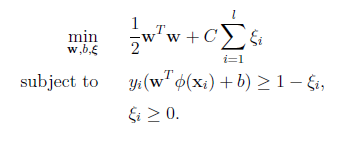
\includegraphics[height=1.15in]{figuras/Imagen1.png}
\end{center}
Los vectores de entrenamiento $x_i$ son mapeados en un espacio dimensional más alto por la función $\phi$. SVM busca un hiper-plano separador lineal con el máximo margen en este espacio dimensional. Consecuentemente, $K(x_i,x_j)\equiv \phi(x_i )^T \phi(x_j)$ se conoce como la función kernel. Cada vez más, nuevas funciones kernel son propuestas por investigadores. Algunas conocidas son los kernel lineal, polinomial, radial basis function (RBF) y sigmoid (Chih-Wei Hsu, Chih-Chung Chang, 2008). 

La información de la actividad cerebral y los patrones que se pueden extraer de la misma tiene una relación no lineal (Davatzikos et al., 2005). El kernel radial basis function (RBF) tiene utilidad cuando la información tiene esta característica. Este kernel asigna muestras de forma no lineal a un espacio dimensional superior para que, a diferencia del kernel lineal, pueda manejar el caso cuando la relación entre los valores objetivos y los atributos no es lineal. Formalmente, este kernel (Chih-Wei Hsu, Chih-Chung Chang, 2008) se describe como:

$$K(x_i,x_j )\equiv exp(-\gamma‖x_i-x_j ‖^2\gamma>0$$

Una de las características más importantes de SVM es que no se calcula a partir de todas las muestras, sino sólo a partir de muestras que se encuentran cerca de la interfaz entre los dos grupos de interés. En nuestro caso, el algoritmo se centra sólo en los patrones de activación que son difíciles de clasificar en respuestas verídicas o no veraces (Davatzikos et al., 2005).

SVM es uno de los algoritmos de machine learning que ha demostrado tener gran competitividad al momento de clasificar grandes sets de datos de altas dimensiones (Tzotsos, 2006). Esto lo hace de gran utilidad al momento de clasificar datos de imágenes. Aun así, el utilizar varios algoritmos de machine learning para analizar datos de imágenes también ha dado resultados alentadores, promoviendo nuevos modelos de clasificación recientemente (Thai, Hai, \& Thuy, 2012). Por ejemplo, se separa imágenes en varias sub-imágenes para ser clasificadas por diversas Artificial Neural Networks (ANN), que luego se compilan para ser procesadas por un SVM. Este tipo de modelos híbridos permiten pensar en modelos complejos para obtener alternativas de interés. 
\subsection{Kernels Lineales y no Lineales}



